\documentclass[11pt,a4paper]{article}

\usepackage[utf8]{inputenc}
\usepackage[T1]{fontenc}
\usepackage[margin=2.5cm]{geometry}
\usepackage{amsmath,amssymb,bm}
\usepackage{booktabs}
\usepackage{array}
\usepackage{enumerate}
\usepackage{xcolor}
\usepackage{hyperref}
\usepackage{tikz}

\hypersetup{colorlinks=true, linkcolor=blue, urlcolor=blue}

\newcommand{\points}[1]{\textbf{(#1\,\%)}}
\newcommand{\subpoints}[1]{\textit{(#1\,\%)}}

\title{TMA4268 Statistical Learning V2026\\[0.3em]
\large Mock Exam 3 (estimated final exam)}
\author{Compiled by Claude for Anders Bekkevard\\[0.2em]
\small Based on the Apr 28 exam-review lecture, the 2023--2025 finals, and the prof's stated scope rule}
\date{Mock for: May 18, 2026 (real exam date)}

\begin{document}
\maketitle

\noindent\fbox{\parbox{\dimexpr\textwidth-2\fboxsep-2\fboxrule}{%
\textbf{Instructions.}
\begin{itemize}
  \item \textbf{Duration:} 4 hours. \textbf{Open book.} Permitted aids: ISLP (2nd ed.), one handwritten A5 sheet of notes, calculator.
  \item \textbf{No code required.} Write answers as math, plain English, or pseudocode. Do \emph{not} memorize R/Python package names.
  \item \textbf{Show your work} --- partial credit is generously available, including when calculator slips spoil a numeric answer but the setup is correct.
  \item \textbf{No negative scoring.} Always answer, even when unsure.
  \item \textbf{If a question seems broken or ambiguous}, state the assumption you are making in one short sentence and proceed.
  \item Total: \textbf{100 points = 100\,\%}. Per-problem weights given in parentheses.
\end{itemize}}}

\vspace{0.6em}
\noindent\textbf{Grade boundaries (NTNU \emph{prosentvurderingsmetoden}, advisory):}
A: 89--100\,\% \quad B: 77--88\,\% \quad C: 65--76\,\% \quad D: 53--64\,\% \quad E: 41--52\,\% \quad F: 0--40\,\%.

\vspace{1em}
\hrule
\vspace{1em}

%=========================================================
\section*{Problem 1 \points{10} --- Fill-in-the-blank concepts}
%=========================================================

\noindent Read the passage below and pick the best word or phrase for each blank from the choices in parentheses. Each correct fill is worth $1$\,\%.

\bigskip

In supervised statistical learning we typically distinguish between methods that produce an explicit functional form for the relationship between predictors and response, called \underline{\hspace{2.5cm}}\,(1) (\emph{parametric} / \emph{generative} / \emph{nonparametric} / \emph{regularized}) methods, and methods that estimate the relationship more flexibly without assuming such a form, called \underline{\hspace{2.5cm}}\,(2) (\emph{parametric} / \emph{nonparametric} / \emph{linear} / \emph{Bayesian}) methods.

A central concept of the course was that the expected squared test error of a fitted model can be written as the sum of three pieces: a squared bias, a variance, and an \underline{\hspace{2.5cm}}\,(3) (\emph{irreducible} / \emph{reducible} / \emph{regularized} / \emph{validated}) component that does not vanish as we collect more training data. Methods such as ridge regression and lasso are referred to as \underline{\hspace{2.5cm}}\,(4) (\emph{shrinkage} / \emph{boosting} / \emph{generative} / \emph{kernel}) methods because they shrink coefficients toward zero. Of these two, \underline{\hspace{2.5cm}}\,(5) (\emph{ridge} / \emph{lasso} / \emph{both} / \emph{neither}) can produce a model in which some coefficients are exactly zero, and is therefore the natural choice when one also wants automatic variable selection.

When the goal is to estimate the prediction error of a fitted model honestly, we use a resampling technique. The simplest is the validation-set approach; a more reliable variant that splits the training data into $k$ roughly equal pieces and rotates which piece serves as held-out data is called \underline{\hspace{2.5cm}}\,(6) (\emph{k-fold cross-validation} / \emph{the bootstrap} / \emph{leave-one-out cross-validation} / \emph{nested CV}). The lecturer in this course generally prefers this technique to penalty-based criteria such as AIC because the latter rely on \underline{\hspace{2.5cm}}\,(7) (\emph{distributional assumptions} / \emph{shrinkage} / \emph{regularization} / \emph{cross-validation}) that often fail in practice.

For non-linear regression we discussed methods that allow each predictor to enter the model through its own non-linear shape and are then summed; this family is called \underline{\hspace{2.5cm}}\,(8) (\emph{generalized additive models} / \emph{principal components} / \emph{convolutional networks} / \emph{boosted trees}).

Finally, in unsupervised learning we discussed two main families. One reduces the dimensionality of the data by finding orthogonal directions of maximal variance and is called \underline{\hspace{2.5cm}}\,(9) (\emph{principal component analysis} / \emph{lasso} / \emph{partial least squares} / \emph{neural networks}); another partitions the observations into groups, of which the agglomerative variant produces a tree-like structure called a \underline{\hspace{2.5cm}}\,(10) (\emph{dendrogram} / \emph{biplot} / \emph{scree plot} / \emph{decision tree}).

\vfill\eject

%=========================================================
\section*{Problem 2 \points{28} --- Multiple choice, true/false, and short numeric}
%=========================================================

For each subproblem, write \emph{True/False} for each statement (or the requested numeric answer). For true/false subproblems you may add a one-sentence justification, but only if you think it helps; do not write essays.

\subsection*{a) Bias--variance and double descent \subpoints{3}}
Mark each statement as true or false.
\begin{enumerate}[(i)]
  \item As the flexibility of a fitted model is increased, its squared bias tends to decrease while its variance tends to increase.
  \item The bias--variance decomposition $\mathbb{E}[(y_0-\hat f(x_0))^2] = \mathrm{Bias}^2 + \mathrm{Var} + \sigma^2$ is an algebraic identity that holds for any fitted model $\hat f$.
  \item In the over-parameterized regime where the number of model parameters $p$ is much larger than $n$, a model that fits the training data perfectly cannot generalize to new data.
  \item In a regression setting in which $\sigma^2$ is large, a more flexible model is generally preferable because it can chase down more of the noise.
\end{enumerate}

\subsection*{b) Cross-validation variants \subpoints{3}}
Mark each statement as true or false.
\begin{enumerate}[(i)]
  \item Leave-one-out cross-validation (LOOCV) generally has lower bias but higher variance than $5$-fold cross-validation as an estimator of test error.
  \item The validation-set approach is the same as $2$-fold cross-validation.
  \item For ordinary least squares, LOOCV can be computed without refitting the model $n$ times by exploiting the diagonal of the hat matrix.
  \item In a feature-selection-then-CV pipeline, it is permissible to use the response $y$ to filter the predictors \emph{once}, before any cross-validation, as long as the CV is then run on the resulting reduced predictor set.
\end{enumerate}

\subsection*{c) Neural network parameters and forward pass \subpoints{4}}
Suppose you build a fully-connected feed-forward neural network with:
\begin{itemize}
  \item $6$ input variables,
  \item one hidden layer of $8$ neurons (with biases, ReLU activations),
  \item one hidden layer of $4$ neurons (with biases, ReLU activations),
  \item one output layer of $2$ neurons (with biases, softmax outputs).
\end{itemize}

\begin{enumerate}[(i)]
  \item \subpoints{2} How many parameters does this network have in total, \emph{including all bias terms}? Show the layer-by-layer breakdown.
  \item \subpoints{2} A neuron in the \emph{first} hidden layer has weights $w = (0.5,\,-1.0,\,0.2,\,1.0,\,-0.5,\,0.3)$ and bias $b = -0.1$. Its inputs on a given observation are $x = (1,\,0,\,2,\,-1,\,1,\,3)$. Using a \emph{sigmoid} activation $\sigma(z) = 1/(1+e^{-z})$, compute the output of this neuron, rounded to three decimals.
\end{enumerate}

\subsection*{d) Odds, log-odds, interaction \subpoints{3}}
\begin{enumerate}[(i)]
  \item \subpoints{1} A patient has probability $p = 0.05$ of an adverse event. What are the odds of that event?
  \item \subpoints{1} A model reports odds $= 4$ for a particular outcome. What is the corresponding probability?
  \item \subpoints{1} In a logistic regression model with the interaction term \texttt{bmi:smokerYes}, the fitted coefficients are $\hat\beta_{\texttt{bmi}}=0.02$ and $\hat\beta_{\texttt{bmi:smokerYes}}=0.10$. By what factor do the odds of the response event change for a \emph{smoker} when \texttt{bmi} increases by one unit, holding all other predictors fixed? (One numeric value, two decimals.)
\end{enumerate}

\subsection*{e) Splines and degrees of freedom \subpoints{3}}
Mark each statement as true or false.
\begin{enumerate}[(i)]
  \item A cubic regression spline with $K$ interior knots consumes $K+4$ parameters (including the intercept).
  \item A natural cubic spline with $K$ interior knots consumes \emph{fewer} parameters than a plain cubic spline with the same number of knots, because the natural spline is constrained to be linear outside the boundary knots.
  \item For a cubic regression spline, the third derivative is continuous at every knot.
  \item Adding more knots to a regression spline typically makes the fit \emph{less} flexible.
\end{enumerate}

\subsection*{f) Principal component analysis \subpoints{5}}
You perform PCA on a dataset with five \textbf{standardized} variables $X_1,\dots,X_5$ and obtain the following decomposition:
\begin{center}\small
\begin{tabular}{lcc}
\toprule
\textbf{PC} & \textbf{Eigenvalue} & \textbf{PVE} \\
\midrule
PC1 & $2.1$ & $0.42$ \\
PC2 & $1.4$ & $0.28$ \\
PC3 & $0.8$ & $0.16$ \\
PC4 & $0.5$ & $0.10$ \\
PC5 & $0.2$ & $0.04$ \\
\bottomrule
\end{tabular}
\end{center}

The loading vector for the first principal component (entries rounded to two decimal places) is
$$\phi_1 = (\,0.55,\;\, 0.45,\;\, -0.40,\;\, 0.30,\;\, -0.50\,)^\top.$$

A new observation has standardized values $x^* = (\,1.5,\;\, -1,\;\, 0.5,\;\, 2,\;\, -0.5\,)^\top$.

\begin{enumerate}[(i)]
  \item \subpoints{1} What is the total variance in the standardized data?
  \item \subpoints{1} What proportion of the total variance is explained by PC1 and PC2 together?
  \item \subpoints{1} How many principal components must be retained to capture at least $95\%$ of the total variance?
  \item \subpoints{1} Compute the score $z^*_1$ of the new observation on PC1.
  \item \subpoints{1} Which one variable contributes \emph{most strongly} to PC1, in absolute terms?
\end{enumerate}

\subsection*{g) Bootstrap \subpoints{3}}
\begin{enumerate}[(i)]
  \item \subpoints{1} For a sample of size $n=8$, what is the probability that a particular original observation is included in a given bootstrap sample? (Numeric, three decimals.)
  \item \subpoints{1} What does this probability tend to as $n \to \infty$? (Both an exact symbolic expression and a numeric approximation.)
  \item \subpoints{1} Mark each of the following as true or false. (A) Bootstrap samples are drawn from the original data \emph{with} replacement; (B) The bootstrap can be used to correct for bias in the original estimator; (C) A single bootstrap sample is informative about the sampling distribution of an estimator.
\end{enumerate}

\subsection*{h) Random forests and out-of-bag error \subpoints{2}}
Mark each statement as true or false.
\begin{enumerate}[(i)]
  \item In a random forest, the standard default for the number of predictors sampled at each split is $m = \sqrt{p}$ for classification and $m = p/3$ for regression.
  \item The number of trees $B$ in a random forest is a tuning parameter that should be chosen by cross-validation.
  \item The out-of-bag (OOB) error of a random forest provides an estimate of test error \emph{without} needing a separate held-out set, because each observation is left out of approximately $1/3$ of the bootstrap samples.
  \item In a random forest, the individual trees are typically grown deep and \emph{unpruned}; variance reduction is provided by averaging across trees rather than by per-tree pruning.
\end{enumerate}

\subsection*{i) $K$-means clustering \subpoints{2}}
Mark each statement as true or false.
\begin{enumerate}[(i)]
  \item The $K$-means objective is to minimize the sum of within-cluster squared Euclidean distances of every point to its cluster mean.
  \item The number of clusters $K$ is determined automatically by the $K$-means algorithm.
  \item Because the $K$-means algorithm depends on a random initialization of the cluster centroids, it is recommended to run it several times from different initializations and pick the solution with the lowest within-cluster sum of squares.
  \item The $K$-means algorithm produces a hierarchy of clusterings that can be cut at any level to obtain different numbers of clusters.
\end{enumerate}

\vfill\eject

%=========================================================
\section*{Problem 3 \points{16} --- Theory and hand calculations}
%=========================================================

\subsection*{a) The mathy one --- LDA decision boundary \subpoints{8}}

Consider a binary classification problem with two classes $0$ and $1$. Assume that the class-conditional densities are bivariate normal with class-specific means but a \emph{shared} covariance matrix:
$$\mathbf{X} \mid Y=k \;\sim\; \mathcal{N}_2(\boldsymbol\mu_k,\, \boldsymbol\Sigma), \qquad k = 0, 1,$$
with class priors $\pi_0$ and $\pi_1 = 1-\pi_0$.

For the numerical part below, take
$$\boldsymbol\mu_0 = \begin{pmatrix}1\\1\end{pmatrix}, \quad
  \boldsymbol\mu_1 = \begin{pmatrix}3\\5\end{pmatrix}, \quad
  \boldsymbol\Sigma = \begin{pmatrix}4 & 1\\1 & 4\end{pmatrix}, \quad
  \pi_0 = \pi_1 = 0.5.$$

\begin{enumerate}[(i)]
  \item \subpoints{2} State, in one or two sentences each, the two key modelling assumptions of LDA. State also one practical reason why one might prefer LDA to QDA when the number of training observations per class is small.
  \item \subpoints{3} Starting from $\log(\pi_k f_k(\mathbf{x}))$, derive the LDA discriminant function
    $$\delta_k(\mathbf{x}) \;=\; \mathbf{x}^\top \boldsymbol\Sigma^{-1}\boldsymbol\mu_k \;-\; \tfrac{1}{2}\boldsymbol\mu_k^\top \boldsymbol\Sigma^{-1}\boldsymbol\mu_k \;+\; \log\pi_k.$$
    Be \emph{explicit} about which terms in the log-likelihood do and do not depend on $k$, and explain why $\delta_k(\mathbf{x})$ is \emph{linear} in $\mathbf{x}$.
  \item \subpoints{2} Using the numerical values above, derive the equation of the LDA decision boundary in the form $a x_1 + b x_2 = c$. (You may use $\boldsymbol\Sigma^{-1} = \frac{1}{15}\begin{pmatrix}4 & -1\\-1 & 4\end{pmatrix}$.)
  \item \subpoints{1} If you instead allowed the two classes to have \emph{different} covariance matrices $\boldsymbol\Sigma_0 \neq \boldsymbol\Sigma_1$, the resulting decision boundary would no longer be linear. What \emph{shape} does it take, and what is the name of this method?
\end{enumerate}

\subsection*{b) Hierarchical clustering by hand \subpoints{5}}

Four observations have the following Euclidean dissimilarity matrix:
$$D = \begin{pmatrix}
0 & 3 & 7 & 8 \\
3 & 0 & 5 & 6 \\
7 & 5 & 0 & 4 \\
8 & 6 & 4 & 0 \\
\end{pmatrix}.$$

\begin{enumerate}[(i)]
  \item \subpoints{3} Sketch the dendrogram produced by hierarchical clustering with \emph{single} linkage. Label the leaves $1, 2, 3, 4$, indicate the fusion height of each merge on a properly labelled $y$-axis, and show the recomputed dissimilarity matrix after the first merge.
  \item \subpoints{1} If you instead used \emph{complete} linkage on the same matrix, the order of the merges would be unchanged, but the height of the \emph{final} fusion (when all four observations are joined) would differ. Compute the final fusion height under complete linkage and explain in one sentence why it differs from the single-linkage answer.
  \item \subpoints{1} Suppose you cut the single-linkage dendrogram at height $4.5$. How many clusters do you obtain, and which observations are in each cluster?
\end{enumerate}

\subsection*{c) The bias--variance decomposition and double descent \subpoints{3}}

\begin{enumerate}[(i)]
  \item \subpoints{2} Let $y_0 = f(x_0) + \varepsilon$ with $\mathbb{E}[\varepsilon] = 0$ and $\mathrm{Var}(\varepsilon) = \sigma^2$, and let $\hat f$ be a model fit on a random training set. Write down the bias--variance decomposition of the expected squared test error
$$\mathbb{E}\!\left[(y_0 - \hat f(x_0))^2\right]$$
as a sum of three terms. \emph{Identify each term by name} and \emph{state what randomness the expectations are taken over}.
  \item \subpoints{1} Below are two stylized profiles of test MSE as you increase the flexibility of the fitted model (e.g.\ the degree of a polynomial regression).
  \begin{itemize}
    \item \textbf{Profile A:} test MSE drops, hits a single minimum, and then rises monotonically (the classical U-shape).
    \item \textbf{Profile B:} test MSE drops, then climbs to a peak around the point where the number of fitted parameters equals the training set size, and then \emph{descends a second time} to a value below the original minimum.
  \end{itemize}
  Identify Profile B by its standard name, and explain in one or two sentences why both profiles are consistent with the same exact bias--variance decomposition. (Hint: think about what the optimization is implicitly doing once there are infinitely many zero-training-error solutions.)
\end{enumerate}

\vfill\eject

%=========================================================
\section*{Problem 4 \points{22} --- Data analysis: insurance premiums
%=========================================================
}

A health insurer records $n = 900$ customers' annual insurance premium \texttt{charges} (in $1000$\,EUR). The available predictors are:
\begin{itemize}
  \item \texttt{age} --- age in years (continuous, $18$--$65$);
  \item \texttt{bmi} --- body-mass index, $\mathrm{kg}/\mathrm{m}^2$ (continuous, $16$--$50$);
  \item \texttt{children} --- number of dependent children (count, $0$--$5$);
  \item \texttt{smoker} --- categorical: \emph{no} (reference), \emph{yes};
  \item \texttt{sex} --- categorical: \emph{female} (reference), \emph{male};
  \item \texttt{region} --- categorical, $4$ levels: \emph{northeast} (reference), \emph{northwest}, \emph{southeast}, \emph{southwest}.
\end{itemize}

The data are split $600/300$ into a training set and a test set.

\subsection*{a) Linear regression with interaction \subpoints{7}}

The course staff fit, on the training set, the linear model
$$\texttt{charges} \,\sim\, \texttt{age} + I(\texttt{age}^2) + \texttt{bmi} + \texttt{smoker} + \texttt{bmi:smoker} + \texttt{sex} + \texttt{region} + \texttt{children},$$
where \texttt{bmi:smoker} denotes the (continuous $\times$ binary) interaction between \texttt{bmi} and \texttt{smoker}. The fitted output is:

\begin{center}\small
\begin{tabular}{lcccc}
\toprule
 & \textbf{Estimate} & \textbf{Std.\ Error} & \textbf{t-value} & \textbf{Pr($>|t|$)} \\
\midrule
(Intercept)              & $-2.50$  & $1.80$    & $-1.39$  & $0.165$ \\
\texttt{age}             & $-0.05$  & $0.10$    & $-0.50$  & $0.617$ \\
$I(\texttt{age}^2)$      & $0.0040$ & $0.0010$  & $4.00$   & $<0.001$ \\
\texttt{bmi}             & $0.10$   & $0.05$    & $2.00$   & $0.046$ \\
\texttt{smoker\_yes}     & $-22.50$ & $5.00$    & $-4.50$  & $<0.001$ \\
\texttt{bmi:smoker\_yes} & $1.45$   & $0.18$    & $8.06$   & $<0.001$ \\
\texttt{sex\_male}       & $0.10$   & $0.21$    & $0.48$   & $0.633$ \\
\texttt{region\_NW}      & $-0.45$  & $0.30$    & $-1.50$  & $0.134$ \\
\texttt{region\_SE}      & $0.18$   & $0.30$    & $0.60$   & $0.549$ \\
\texttt{region\_SW}      & $-0.62$  & $0.30$    & $-2.07$  & $0.039$ \\
\texttt{children}        & $0.55$   & $0.10$    & $5.50$   & $<0.001$ \\
\bottomrule
\end{tabular}
\end{center}

\noindent Multiple $R^2 = 0.78$,\quad Adjusted $R^2 = 0.776$.\quad Residual standard error: $4.10$ on $589$ d.f.

\begin{enumerate}[(i)]
  \item \subpoints{1} How many parameters does this model estimate, including the intercept?
  \item \subpoints{2} For a \emph{non-smoker}, by how much (in EUR) does an increase of one BMI unit change the predicted annual charges, holding all other predictors fixed? Repeat the calculation for a \emph{smoker}. (Two numeric answers; remember that \texttt{charges} is in $1000$\,EUR.)
  \item \subpoints{2} Briefly explain why the main-effect coefficient on \texttt{smoker\_yes} alone (here $-22.50$) is \emph{not} a useful summary of the average effect of being a smoker on premiums. (Mention the role of the interaction.)
  \item \subpoints{1} An analyst wants to test whether \texttt{region} is jointly relevant after controlling for the other predictors. State \textbf{which test} you would use and write the null hypothesis. (You do \emph{not} need to compute the test statistic by hand.)
  \item \subpoints{1} The model reports $R^2 = 0.78$ and adjusted $R^2 = 0.776$. Briefly comment on what the closeness of these two numbers suggests.
\end{enumerate}

\subsection*{b) Ridge regression with $10$-fold cross-validation \subpoints{5}}

The same predictors are now fed (after standardization) into a ridge regression, with the penalty parameter $\lambda$ chosen by $10$-fold cross-validation. The CV-MSE profile is:

\begin{center}
\begin{tikzpicture}[scale=0.85]
  \draw[->] (0,0) -- (8,0) node[right] {$\log\lambda$};
  \draw[->] (0,0) -- (0,4) node[above] {CV-MSE};

  \draw[smooth, thick, blue] plot[domain=0.4:7.6] (\x, {3.6 + 0.04*(\x-1.2)*(\x-1.2)*(\x-1.2) + 0.18*(\x-1.2)*(\x-1.2) - 0.5*(\x-1.2)});
  \draw[dashed] (1.2,0) -- (1.2, 3.4) node[above] {\small $\hat\lambda_{\min}$};
  \draw[dashed] (3.0,0) -- (3.0, 3.5) node[above] {\small $\hat\lambda_{1\mathrm{SE}}$};

  \foreach \x in {0,2,4,6}
    \draw (\x, 0.06) -- (\x, -0.06) node[below] {\x};
  \foreach \y in {0,1,2,3,4}
    \draw (-0.06, \y) -- (0.06, \y) node[left,xshift=-0.1cm] {\y};

  \node at (4, 4.5) {\small CV curve};
\end{tikzpicture}
\end{center}

\noindent (You may take, on the same test set as in part (a):
test MSE for OLS $= 38.0$;\quad test MSE for ridge at $\hat\lambda_{\min} = 38.4$;\quad test MSE for ridge at $\hat\lambda_{1\mathrm{SE}} = 39.1$.)

\begin{enumerate}[(i)]
  \item \subpoints{1} Why is it important to standardize the predictors \emph{before} fitting ridge regression? Give a one-sentence explanation.
  \item \subpoints{1} Write down the ridge regression objective function, and explain (in words) what happens to $\hat\beta^R_\lambda$ as $\lambda \to 0$ and as $\lambda \to \infty$.
  \item \subpoints{2} State the \emph{one-standard-error rule} precisely, and give one reason a practitioner might prefer $\hat\lambda_{1\mathrm{SE}}$ over $\hat\lambda_{\min}$.
  \item \subpoints{1} On this dataset, ridge at $\hat\lambda_{\min}$ gives test MSE $=38.4$ while OLS gives $38.0$. Briefly interpret this comparison in bias--variance terms: what does it suggest about the predictors in this dataset?
\end{enumerate}

\subsection*{c) GAM with splines \subpoints{5}}

A generalized additive model is fit on the same training set:
$$\texttt{charges} \,=\, \beta_0 \,+\, s(\texttt{age},\, \mathrm{df}=4) \,+\, \mathrm{bs}(\texttt{bmi},\, \text{knots}=\{25, 30, 35\}) \,+\, \beta_{\texttt{smoker}}\cdot \texttt{smoker} \,+\, g(\texttt{region}) \,+\, \beta_{\texttt{kids}}\cdot \texttt{children} \,+\, \varepsilon,$$
where $s(\cdot,\mathrm{df}=4)$ denotes a smoothing spline with $4$ effective degrees of freedom (intercept removed), $\mathrm{bs}(\cdot)$ denotes a cubic regression spline (intercept removed), and $g(\texttt{region})$ uses dummy coding as in part (a).

\begin{enumerate}[(i)]
  \item \subpoints{2} How many degrees of freedom does this GAM consume in total (including the global intercept)? Give a brief term-by-term breakdown.
  \item \subpoints{1} What is the structural assumption that the GAM makes about the relationship between, say, \texttt{age} and \texttt{bmi}, and in what sense is this a \emph{limitation} compared to (for example) a regression tree?
  \item \subpoints{2} Suppose the GAM achieves test MSE $= 32.5$ on the same test set as part (a)/(b). Compare this to the OLS result of $38.0$. What does the gap suggest about the underlying relationship between predictors and \texttt{charges}, and which predictor would you suspect contributes most to the improvement (briefly justify by reference to the model output in part (a))?
\end{enumerate}

\subsection*{d) Tree boosting \subpoints{5}}

Finally a gradient-boosted regression tree is fit on the same training data; it achieves test MSE $= 26.8$.

\begin{enumerate}[(i)]
  \item \subpoints{2} Gradient boosting has three main hyperparameters: the number of trees $B$, the interaction depth $d$ (per-tree size), and the shrinkage / learning rate $\nu$. For each, briefly say how you would choose its value and how it qualitatively affects the bias--variance behaviour of the resulting ensemble.
  \item \subpoints{1} For a \emph{random forest}, the number of trees $B$ is \emph{not} a tuning parameter and one simply uses ``enough'' of them. For \emph{boosting}, $B$ \emph{is} a real tuning parameter. Briefly explain why this difference exists.
  \item \subpoints{2} Comparing the test MSEs --- boosting $26.8$, GAM $32.5$, OLS $38.0$ --- what does the ranking suggest about the structure of the relationship between predictors and \texttt{charges}? If you also wanted \emph{interpretation} (which predictors matter, and roughly in which direction), what additional diagnostic would you compute from the boosted model?
\end{enumerate}

\vfill\eject

%=========================================================
\section*{Problem 5 \points{24} --- Data analysis: stroke risk classification}
%=========================================================

A teaching hospital records $n = 4000$ patients followed for five years; the binary response \texttt{stroke} is $1$ if the patient suffered a stroke during follow-up and $0$ otherwise. The available predictors are:
\begin{itemize}
  \item \texttt{age} --- age in years (continuous);
  \item \texttt{avg\_glucose} --- average blood glucose (continuous, $\mathrm{mg/dL}$);
  \item \texttt{bmi} --- body-mass index (continuous);
  \item \texttt{hypertension} --- binary $0/1$ indicator;
  \item \texttt{heart\_disease} --- binary $0/1$ indicator;
  \item \texttt{smoking\_status} --- categorical, $4$ levels: \emph{never} (reference), \emph{former}, \emph{current}, \emph{unknown}.
\end{itemize}

The data are split $70/30$ into training ($2800$) and test ($1200$) sets. Among the test set there are $120$ true strokes and $1080$ true non-strokes.

\subsection*{a) Logistic regression \subpoints{8}}

A logistic regression model is fit on the training set with the predictors above (no interactions). The fitted output is:

\begin{center}\small
\begin{tabular}{lcccc}
\toprule
 & \textbf{Estimate} & \textbf{Std.\ Error} & \textbf{z-value} & \textbf{Pr($>|z|$)} \\
\midrule
(Intercept)            & $-8.50$   & $0.50$     & $-17.00$  & $<0.001$ \\
\texttt{age}           & $0.073$   & $0.005$    & $14.60$   & $<0.001$ \\
\texttt{avg\_glucose}  & $0.005$   & $0.0008$   & $6.25$    & $<0.001$ \\
\texttt{bmi}           & $-0.005$  & $0.012$    & $-0.42$   & $0.674$  \\
\texttt{hypertension}  & $0.45$    & $0.12$     & $3.75$    & $<0.001$ \\
\texttt{heart\_disease}& $0.50$    & $0.13$     & $3.85$    & $<0.001$ \\
\texttt{smoking\_former}  & $0.18$ & $0.15$     & $1.20$    & $0.230$  \\
\texttt{smoking\_current} & $0.32$ & $0.16$     & $2.00$    & $0.046$  \\
\texttt{smoking\_unknown} & $0.05$ & $0.18$     & $0.28$    & $0.781$  \\
\bottomrule
\end{tabular}
\end{center}

\begin{enumerate}[(i)]
  \item \subpoints{2} By what factor do the odds of stroke multiply for each one-year increase in \texttt{age}, holding all other predictors fixed? (Numeric answer, to three decimals.) State briefly in words how the magnitude should be interpreted.
  \item \subpoints{3} Consider a patient with the following profile: \texttt{age}\,$=68$, \texttt{avg\_glucose}\,$=180$, \texttt{bmi}\,$=28$, \texttt{hypertension}\,$=1$, \texttt{heart\_disease}\,$=0$, \texttt{smoking\_status}\,$=$\,\emph{current}. Compute the predicted probability $\hat p$ of stroke for this patient. Show your work, including the linear predictor $\hat\eta$ and the sigmoid step.
  \item \subpoints{1} At a default classification threshold of $\hat p = 0.5$, would this patient be predicted to have a stroke? Justify in one sentence.
  \item \subpoints{2} Define, \emph{in words appropriate to this specific problem}, what \emph{sensitivity} and \emph{specificity} mean for the stroke classifier. Briefly comment on what it would mean clinically if a screening tool had high sensitivity but low specificity.
\end{enumerate}

\subsection*{b) LDA vs.\ QDA \subpoints{6}}

LDA and QDA are also fit on the same training set, using the same predictors as in part (a). On the test set they produce the following confusion matrices.

\begin{center}\small
\textbf{LDA} \\[0.3em]
\begin{tabular}{c|cc}
 & \textbf{Predicted: stroke} & \textbf{Predicted: no stroke} \\ \hline
\textbf{Actual: stroke}    & $50$  & $70$  \\
\textbf{Actual: no stroke} & $100$ & $980$ \\
\end{tabular}\\[0.6em]

\textbf{QDA} \\[0.3em]
\begin{tabular}{c|cc}
 & \textbf{Predicted: stroke} & \textbf{Predicted: no stroke} \\ \hline
\textbf{Actual: stroke}    & $75$  & $45$  \\
\textbf{Actual: no stroke} & $250$ & $830$ \\
\end{tabular}
\end{center}

\begin{enumerate}[(i)]
  \item \subpoints{2} Compute the sensitivity, specificity, and overall test error rate of the LDA classifier.
  \item \subpoints{2} Compute the same three quantities for the QDA classifier.
  \item \subpoints{2} Briefly compare the two classifiers. State which one you would prefer and \emph{on which criterion}, justifying your answer with reference to (a) the modelling difference between LDA and QDA, and (b) the medical context (cost of a false negative vs.\ a false positive).
\end{enumerate}

\subsection*{c) A tree-based competitor: random forest \subpoints{5}}

You also fit a \emph{random forest} with $B = 500$ trees and $\mathtt{mtry} = 3$ on the training data. On the test set it produces:

\begin{center}\small
\begin{tabular}{c|cc}
 & \textbf{Predicted: stroke} & \textbf{Predicted: no stroke} \\ \hline
\textbf{Actual: stroke}    & $65$  & $55$  \\
\textbf{Actual: no stroke} & $130$ & $950$ \\
\end{tabular}
\end{center}

\begin{enumerate}[(i)]
  \item \subpoints{1} Justify briefly the choice $\mathtt{mtry} = 3$. (Recall: there are $6$ predictors at the tree-fitting stage.)
  \item \subpoints{1} Compute the test sensitivity, specificity, and error rate.
  \item \subpoints{1} Briefly explain what the \emph{out-of-bag (OOB) error} is and why it is a useful diagnostic for a random forest.
  \item \subpoints{2} The variable-importance plot from this forest shows \texttt{age} and \texttt{avg\_glucose} as having far higher importance than the other predictors. State (a) what a variable-importance plot from a random forest \emph{shows}, and (b) what kind of question it \emph{cannot} answer.
\end{enumerate}

\subsection*{d) ROC and AUC \subpoints{3}}

A schematic ROC curve for the logistic regression of part (a), together with the diagonal of chance, is sketched below.

\begin{center}
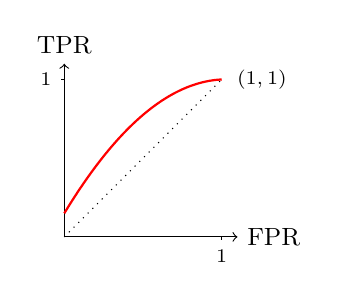
\begin{tikzpicture}[scale=2.0]
  \draw[->] (0,0) -- (1.1,0) node[right] {\small FPR};
  \draw[->] (0,0) -- (0,1.1) node[above] {\small TPR};
  \draw[dotted] (0,0) -- (1,1);
  \draw[smooth, thick, red] plot[domain=0:1] (\x, {1-(1-\x)*(1-\x)*0.85 - 0.05*(1-\x)*\x});
  \node at (1,1) [right=2pt] {\scriptsize $(1,1)$};
  \draw (0,1) -- (-0.02,1) node[left] {\scriptsize 1};
  \draw (1,0) -- (1,-0.02) node[below] {\scriptsize 1};
\end{tikzpicture}
\end{center}

The model achieves AUC $= 0.84$.

\begin{enumerate}[(i)]
  \item \subpoints{1} What does AUC $= 0.84$ \emph{mean} in plain English (i.e.\ beyond ``the area under the ROC curve'')? Frame your answer in terms of randomly chosen positive and negative cases.
  \item \subpoints{1} A clinician argues that the default threshold of $\hat p = 0.5$ misses too many true stroke cases. If the threshold is lowered from $0.5$ to $0.3$, in which direction will sensitivity and specificity move?
  \item \subpoints{1} On the ROC curve sketched above, in which direction does the operating point move when the threshold is lowered?
\end{enumerate}

\subsection*{e) Class imbalance \subpoints{2}}

In the full dataset, only about $5\%$ of patients suffer a stroke during the five-year follow-up.

\begin{enumerate}[(i)]
  \item \subpoints{1} A naive classifier that always predicts ``no stroke'' would achieve a test error rate of approximately what value? Justify in one sentence.
  \item \subpoints{1} In light of (i), comment on whether the test error rate is the most appropriate metric for choosing between classifiers on this dataset. What metric (or pair of metrics) would you privilege instead, and why?
\end{enumerate}

\vspace{1em}
\hrule
\vspace{0.5em}

\noindent\textbf{End of exam.} \quad Total: $10 + 28 + 16 + 22 + 24 = 100$ points.

\end{document}
